
\medskip

Le gros globe de cristal est un trophée attribué au vainqueur de la coupe du monde de ski.

Ce trophée pèse 9 kg et mesure 46 cm de hauteur.

\parbox{0.8\linewidth}{
\begin{enumerate}
\item Le biathlète français Martin Fourcade a remporté le sixième gros globe de cristal de
sa carrière en 2017 à Pyeongchang en Corée du Sud.

Donner approximativement la latitude et la longitude de ce lieu repéré sur la carte
ci-dessous.\end{enumerate}}\hfill
\parbox{0.18\linewidth}{
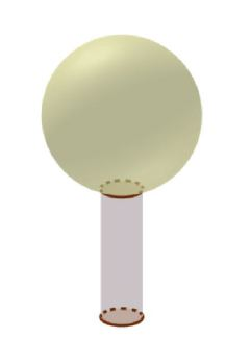
\includegraphics[width=2.5cm]{globe}
}

\medskip

\begin{center}

\psset{unit=0.7cm}
\begin{pspicture}(0,-0.2)(17.2,8.5)
\rput(8.6,4.25){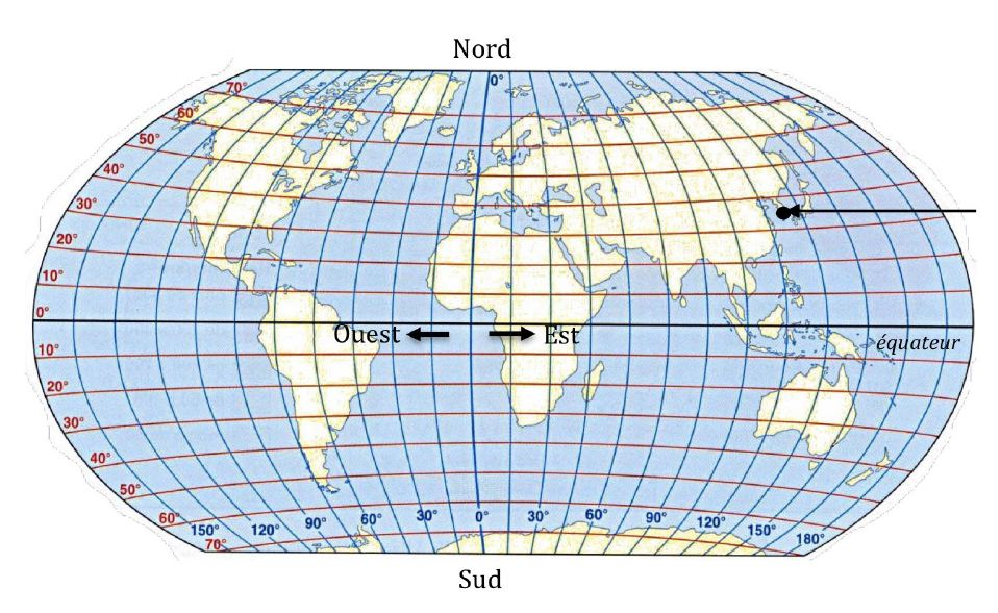
\includegraphics[width=13cm]{mappemonde}}
\rput(8.6,4.25){Nord}\rput(8.6,0.25){Sud}
\uput[r](15,5.7){Pyeongchang}
\end{pspicture}
\end{center}

\medskip

\parbox{0.62\linewidth}{\begin{enumerate}[resume]
\item On considère que ce globe est composé d'un cylindre en cristal de
diamètre 6cm, surmonté d'une boule de cristal. Voir schéma ci -contre.
Montrer qu'une valeur approchée du volume de la boule de ce trophée
est de \np{6371}~cm$^3$.
\item Marie affirme que le volume de la boule de cristal représente environ
90\,\% du volume total du trophée.

A-t-elle raison ?
\end{enumerate}}\hfill \parbox{0.3\linewidth}
{
\psset{unit=0.6cm,arrowsize=2pt 4}
\begin{pspicture}(-0.5,0)(5.3,7.7)
%\psgrid
\psframe(2.8,0.8)(3.7,4.2)
\pscircle(3.25,5.85){1.65}
\psline{<->}(1.3,4.2)(1.3,7.45)\uput[l](1.3,5.8125){23~cm}
\psline{<->}(1.3,0.8)(1.3,4.2)\uput[l](1.3,2.5){23~cm}
\psline[linestyle=dashed](1.2,0.8)(5.3,0.8)
\psline[linestyle=dashed](1.2,4.2)(5.3,4.2)
\psline[linestyle=dashed](1.2,7.45)(5.3,7.45)
\end{pspicture}
}

\medskip

Rappels :

volume d'une boule de rayon $R$ : $V = \frac{4}{3}\pi R^3$

volume d'un cylindre de rayon $r$ et de hauteur $h$ : $V =\pi r^2h$.

\bigskip

